\documentclass[12pt,a4paper]{article}
\usepackage[UTF8]{ctex}
\usepackage[backend=bibtex]{biblatex}
\usepackage{amsmath,amsthm,amssymb,graphicx,multirow,float,caption}
\usepackage{geometry}
\geometry{left=2.54cm, right=2.54cm, top=3.18cm, bottom=3.18cm}
\usepackage{enumitem}
\usepackage{subcaption,booktabs,diagbox}
\setenumerate[1]{itemsep=0pt,partopsep=0pt,parsep=\parskip,topsep=5pt}
\setitemize[1]{itemsep=0pt,partopsep=0pt,parsep=\parskip,topsep=5pt}
\setdescription{itemsep=0pt,partopsep=0pt,parsep=\parskip,topsep=5pt}
\usepackage{adjustbox}
\usepackage[graphicx]{realboxes}
\usepackage{rotating}

\usepackage{titlesec}

\newcommand{\be}[1]{
    \begin{equation}
        #1
    \end{equation}
}

\newcommand{\bfig}[3]{
    \begin{figure}[H]
        \centering
        \includegraphics[width=#1\textwidth]{#2}
        \caption{#3}
    \end{figure}
}

\titleformat{\section}%设置section的样式
{\raggedright\large\bfseries}%右对齐,4号字,加粗
{\thesection .\quad}%标号后面有个点
{0pt}%sep label和title之间的水平距离
{}%标题前没有内容
\title{\vspace{-4cm}\Large 声光效应与光速测量}  %文章标题
\author{\kaishu 学号:202111999064 \hspace{2cm} 姓名:郑力恒}   %作者的名称
\date{实验日期:2024年4月19日}

\begin{document}
\maketitle

\begin{abstract}
    本实验利用扫描干涉仪测量激光的纵模间距及由声光效应产生的0级,1级,2级衍射劈裂;
实验中测得激光的两纵模间距为619.03MHz,验证了超声波作用下纵模的劈裂满足$\Delta \nu=2\Omega$
使用光拍法测得光速的大小为$c=2.76\times 10^8m/s$。
\end{abstract}

\section{引言}

光速是最基本的物理常数之一,其精确测定及特性研究在现代物理学和实验技术中具有重要意义。自十七世纪伽利略首次尝试测量光速以来,各时期科学家们都采用最先进的技术进行光速测量。1849年,法国物理学家斐索成功测得光速,证明了光速可以在实验中测量。1850年,傅科用旋转镜法测得光速 $2.98 \times 10^8 \ \text{m/s}$,推动了光学实验技术的发展。此后,光速测量方法不断改进,获得了数值相近的结果。1970年,激光技术的应用使光速测量达到新的精度,国际计量局在1973年推荐了当前最精确的光速值为 $299,792,458 \pm 1 \ \text{m/s}$。

声光效应是光通过超声波扰动介质时发生衍射的现象,激光的出现极大促进了声光效应的研究和应用。声光效应被广泛用于激光技术、光信号处理和集成光通讯技术中。本实验采用光拍法测定光速,旨在使学生理解光拍频波的概念,了解声光效应原理及驻波法产生声光频移的实验条件和特点,掌握光拍法测量光速的技术。

\section{原理}
\subsection{光拍频波}

根据波的叠加原理,两束传播方向相同、偏振方向相同且频率相差很小的简谐波相叠加即形成拍频波。对于振幅均为 $E_0$,角频率分别为 $\omega_1$ 和 $\omega_2$,且沿相同方向传播的两束单色光(假设沿 $x$ 方向)分别为:
\begin{equation}
\begin{align}
    E_{1} & = E_{0} \cos \left(\omega_{1} t-\frac{\omega_{1} x}{c}+\phi_{1}\right)\\
    E_{2} & = E_{0} \cos \left(\omega_{2} t-\frac{\omega_{2} x}{c}+\phi_{2}\right)
    \end{align}
\end{equation}
它们的叠加为:
\begin{equation}
\begin{align}
    E & = E_{1}+E_{2}\\ & = 2 E_{0} \cos \left(\frac{\omega_{1}+\omega_{2}}{2} t-\frac{\omega_{1}+\omega_{2}}{2} \frac{x}{c}+\frac{\phi_{1}+\phi_{2}}{2}\right) \cos \left(\frac{\omega_{1}-\omega_{2}}{2} t-\frac{\omega_{1}-\omega_{2}}{2} \frac{x}{c}+\frac{\phi_{1}-\phi_{2}}{2}\right)
    \end{align}
    \end{equation}
当 $\omega_1 > \omega_2$ 且 $\Delta \omega = \omega_1 - \omega_2$ 较小时,合成光波是带有低频调制的高频波,其振幅为 $2 E_0 \cos\left( \frac{\Delta \omega}{2} t - \frac{\Delta \omega}{2} \frac{x}{c} + \frac{\phi_1 - \phi_2}{2} \right)$,角频率为 $\frac{\omega_1 + \omega_2}{2}$。由于振幅以频率 $\Delta f = \frac{\Delta \omega}{2\pi}$ 周期性地缓慢变化,我们将合成光波称之为光拍频波,$\Delta f$ 称为拍频。光拍频波的形成和传播如图1所示。

\subsection{拍频信号的检测}

在实验中,我们用光电检测器接收光信号。光电检测器所产生的光电流与接收到的光强(即电场强度 $E$ 的平方)成正比:


\be{I = gE^2}

式中 $g$ 为光电转换系数。由于光的频率极高($f_0 > 10^{14} \ \text{Hz}$),而一般光电器件仅能对 $10^8 \ \text{Hz}$ 以下的光强变化作出响应,因此实际得到的光电流 $I_c$ 近似为响应时间 $\tau$ 内光电检测器接收到的光强的平均。


\be{I_c = \frac{1}{\tau} \int_{t-\tau}^{t} gE^2 \, dt }

式中,高频项平均后为零。光电检测器输出的光电流包括直流和光拍频波两部分。滤去直流部分,即得到频率为 $\Delta f = \frac{\omega_1 - \omega_2}{2\pi}$,初相位为 $\phi_1 - \phi_2$,相位和空间位置有关的简谐拍频信号。

图 2 是拍频光信号 $I_c$ 在某一时刻的空间分布。可见,在某一时刻 $t$,置于不同空间位置的光电检测器将输出不同相位的光电流,因此,用比较相位的方法可以间接测定光速。

假设在测量线上有两点 $x_A$ 和 $x_B$,由(4)式可知,在某一时刻 $t$,当点 $x_A$ 与 $x_B$ 之间的距离等于光拍频波的波长 $\lambda$ 的整数倍时,该两点的相位差为:


\be{\frac{(\omega_1 - \omega_2)}{c} (x_A - x_B) = 2n\pi, \quad n = 1,2,3, \ldots }

考虑到 $\Delta \omega = \omega_1 - \omega_2$,从而:


\be{x_A - x_B = n \frac{c}{\Delta f}, \quad n = 1,2,3, \ldots }

当相邻两个同相位点之间的距离 $x_A - x_B$ 等于光拍频波的波长 $\lambda$,即 $n=1$ 时,由(6)式得:

\be{\lambda = \frac{c}{\Delta f} }

上式说明,只要我们在实验中测出 $\Delta f$ 和 $\lambda$,就可间接确定光速 $c$。

\subsection{利用声光效应产生光拍频波}

声光效应研究光通过声波扰动介质时的散射或衍射现象。衍射光的频率因与超声波频率有关而发生频率移动,从而实现激光束频移。本实验采用驻波法,通过声光效应使 He—Ne 激光器的 632.8nm 谱线产生固定频差,形成光拍频波。

驻波法是使声光介质的厚度为超声波半波长的整数倍,使超声波在介质中反射并形成驻波场,入射激光因此产生多级对称衍射。第 L 级衍射光的角频率为:


\be{\omega_{Lm} = \omega_0 + (L + 2m)\Omega }

其中,$\Omega$ 为超声波角频率,$L, m = 0, \pm1, \pm2, \pm3, \ldots$。

驻波法的特点是,除了不同衍射级的光波产生频移外,同一衍射级的光波中也包含各种不同的频率成分,但各成分的强度互不相同。因此,从每一级衍射光中都能获得光拍频波,而无需通过光路调整混合不同频率的光。因此,驻波法明显优于行波法。在本实验中,我们采用驻波法产生频移,各级衍射光的频率分布和相应的频移量可用扫描干涉仪测量。

本实验的声光效应原理如下。功率信号源输出角频率为 $\Omega$ 的正弦信号加在频移器的晶体压电换能器上,超声波沿 $x$ 方向通过声光介质,使介质内部产生应变,导致介质的折射率在时间和空间上发生周期性变化,形成光栅,入射激光束发生衍射并改变传播方向,产生与超声波频率有关的频移。通过仔细调整光路,可使两束光平行叠加,产生频差为 $\Delta \omega =2 \Omega$ 的光拍频波。


\section{实验}
\subsection{实验仪器}

示波器、扫描干涉仪、数字频率计、光速测量仪、He-Ne激光器

\subsection{实验步骤}

\subsubsection{测量声光效应产生的频移}

光拍频波要求相拍的两束光有确定的频率差。本实验通过声光效应使 He-Ne 激光器的 632.8nm 谱线产生固定频差。先利用扫描干涉仪观察激光器的纵模模式及裂距,测量 0 级、1 级、2 级衍射光的纵模分裂间距。在测量过程中,调节声光晶体的转角、超声波频率和强度,记录不同级次的衍射强度变化以及同级衍射中不同频率信号的强度变化。

\subsubsection{双光束相位比较法测量光速}

将功率信号源输出角频率为 $\Omega$ 的正弦信号加在频移器的晶体压电换能器上,从而产生角频率为 $\Omega$ 的超声波。实验中采用“双光束相位比较法”进行相位比较。光拍频信号进入光电二极管后转化为光拍频电信号,经混频、选频放大,输出到示波器上进行相位比较。

实验中将激光分束为远程光和近程光,通过移动改变内、外侧滑块的位置,调节远程光与近程光的光程差。当改变光程时,示波器上远程光与近程光的波形会发生移动,通过改变远程光的光程使其波形与近程光波形从一次重合平移到另一次重合,此时远程光光程的改变长度 $L$ 即为拍频波长 $\lambda$。

利用此方法可测得光速:


\be{c = \lambda \Delta f = 2\Omega L}


本实验用 LM2000C 型光速测量仪测定光速。驱动晶体振动的信号源频率 $\Omega$ 约为 75MHz。实验中还配备了示波器、共焦球面干涉扫描仪及数字频率计各一台。光源采用氦氖激光器,输出波长为 632.8nm,功率大于 1mW。激光射入声光调制器后,得到具有 2 种以上频率的衍射光。取 $L=1$ 的第一级衍射,其中 $m=0, -1$ 两种能量最强的频率成分叠加,可得到拍频为 $2\Omega$ 的光拍频波。

实验中采用“双光束相位比较法”进行相位比较。光拍频信号进入光电二极管后转化为光拍频电信号,经混频、选频放大,输出到示波器的 Y 输入端。同时,将高频信号源的另一路输出信号作为示波器的外触发信号。

用位相法测拍频波的波长时,电路的不稳定性、信号强度等因素会产生附加相移。若在测量过程中被测信号强度始终保持不变,附加相移主要来自电路的不稳定因素。实验中设置高速旋转的斩波器,交替遮挡半透半反镜 2 的透射光和反射光,使光电二极管接收并显示在示波器上的拍频波信号交替显示近程光路和远程光路的拍频波。斩波器速度足够高时,由于人眼的视觉暂留效应及示波器荧光屏的余辉效应,看起来两个拍频波信号是同时显示的。两路光在很短时间内交替经过同样的电路系统,相互间的相位差仅与两路光的光程差有关,从而消除电路附加相移的影响。实验中通过改变远程光的光程,使其波形与近程光波形重合,此时远程光与近程光的光程差即为拍频波长 $\lambda$。

\section{结果分析与讨论}
\subsection{激光纵模测量}
扫描干涉仪的自由光谱区参数为1800Hz,激光的波长为$632.8nm$。
\subsubsection{无超声波}
观察到三个自由光谱区,每个光谱区内有两个模式,测得这6条谱线的时间坐标如下表:
\begin{table}[H]
    \centering
    \begin{tabular}{|c|c|c|c|c|c|c|}
    \hline
      & 1a   & 1b   & 2a  & 2b   & 3a   & 3b   \\ \hline
    $t/ms$ & -3.2 & -0.9 & 3.3 & 5.25 & 8.85 & 10.7 \\ \hline
    \end{tabular}
    \caption{无超声波时激光模式测量}
    \end{table}
从上表中可平均计算两个模式距离$\Delta t=2.033ms$,自由光谱区距离$\Delta t_{SR}=5.9125ms$,则两个纵模频率差为:
\be{\Delta \nu=\Delta \nu_{SR}\frac{\Delta t}{\Delta t_{SR}}=619.03MHz}
\subsubsection{开启超声波,0级}
在声光效应的作用下,激光出现衍射,不同的衍射级中模式分裂情况不同,模式竞争情况也不同。
对于0级衍射斑,每个纵模分裂为三条谱线。在$\Omega=75.12MHz$的条件下,观察到两个自由光谱区,每个自由光谱区内包含两个纵模分裂出的六条谱线,
测量如下表:
\begin{table}[H]
    \centering
    \begin{tabular}{|c|c|c|c|c|c|c|c|c|c|c|c|c|}
    \hline
      & 1a   & 1b   & 1c  & 1d   & 1e   & 1f   & 2a   & 2b   & 2c   & 2d   & 2e    & 2f    \\ \hline
    $t/ms$ & 1.32 & 1.92 & 2.5 & 3.74 & 4.28 & 4.84 & 8.22 & 8.74 & 9.26 & 10.4 & 10.88 & 11.38 \\ \hline
    \end{tabular}
    \caption{超声波影响下的0级衍射激光模式}
    \end{table}
    从上表中可平均计算出每个纵模分裂出的模式距离$\Delta t=0.555ms$,自由光谱区距离$\Delta t_{SR}=6.71ms$,则每个纵模分裂出的谱线频率差为:
    \be{\Delta \nu=\Delta \nu_{SR}\frac{\Delta t}{\Delta t_{SR}}=148.88MHz}
\subsubsection{开启超声波,1级}
对于1级衍射斑,每个纵模分裂为2条谱线。在$\Omega=75.015MHz$的条件下,观察到两个自由光谱区,每个自由光谱区内包含两个纵模分裂出的4条谱线,
测量如下表:
\begin{table}[H]
    \centering
    \begin{tabular}{|c|c|c|c|c|c|c|c|c|}
    \hline
      & 1a    & 1b    & 1c   & 1d   & 2a   & 2b   & 2c  & 2d \\ \hline
    $t/ms$ & -6.95 & -6.05 & -3.2 & -2.3 & 3.85 & 4.65 & 7.2 & 8  \\ \hline
    \end{tabular}
    \caption{超声波影响下的1级衍射激光模式}
    \end{table}
    从上表中可平均计算出每个纵模分裂出的模式距离$\Delta t=0.85ms$,自由光谱区距离$\Delta t_{SR}=10.6ms$,则每个纵模分裂出的谱线频率差为:
    \be{\Delta \nu=\Delta \nu_{SR}\frac{\Delta t}{\Delta t_{SR}}=144.34MHz}
    \subsubsection{开启超声波,2级}
    对于2级衍射斑,每个纵模分裂为3条谱线。在$\Omega=74.976MHz$的条件下,观察到两个自由光谱区,每个自由光谱区内包含两个纵模分裂出的6条谱线,
测量如下表:
\begin{table}[H]
    \centering
    \begin{tabular}{|c|c|c|c|c|c|c|c|c|c|c|c|c|}
    \hline
      & 1a    & 1b   & 1c    & 1d   & 1e   & 1f   & 2a & 2b   & 2c  & 2d   & 2e   & 2f   \\ \hline
    t & -9.05 & -8.1 & -7.15 & -5.1 & -4.2 & -3.3 & 2  & 2.85 & 3.7 & 5.45 & 6.25 & 7.05 \\ \hline
    \end{tabular}
    \caption{超声波影响下的1级衍射激光模式}
    \end{table}
    从上表中可平均计算出每个纵模分裂出的模式距离$\Delta t=0.9ms$,自由光谱区距离$\Delta t_{SR}=10.7ms$,则每个纵模分裂出的谱线频率差为:
    \be{\Delta \nu=\Delta \nu_{SR}\frac{\Delta t}{\Delta t_{SR}}=151.4019MHz}

    上述测量表明,在超声波作用下纵模分裂出的频率差符合$\Delta \nu=2\Omega$。误差的主要来源为谱线的线宽度较大,在示波器读数的误差较大。
    实验中通过改变超声波的功率,发现随着功率的增大,衍射现象愈加明显,可观察到0级衍射强度减弱,其它次级强度增大。
    通过改变声光晶体的方向,发现各级次衍射的纵模与其劈裂的裂距大小不变,但纵模与其劈裂的光强度的相对大小发生变化。
    \begin{figure}[H]
        \centering
        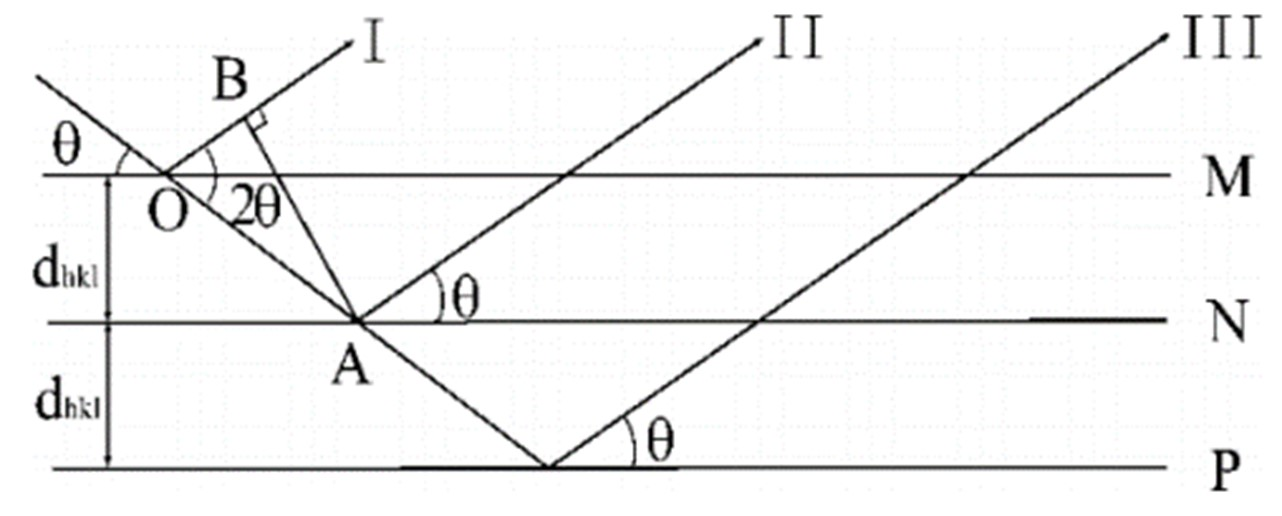
\includegraphics[width=0.7\textwidth]{1.jpg}
        \caption{2级衍射光劈裂在超声波下劈裂示意图}
    \end{figure}
\subsection{光拍法测量光速}
打开斩波器电源,将1级衍射光分为远程光和进程光。之所以选择1级衍射光是因为观察到仅1级衍射光劈裂为两个模式,便于形成频率差稳定的光拍。而0级与2级均有3个模式劈裂,不便进行双光束位相测量。示波器荧光屏上将同时显示远程光和近程光两个正弦波形。注意
斩波器转速适中,过快时示波器上波形可能会左右晃动,过慢时两个波形会闪烁。反复调节
近程、远程光路的等高共轴,使得示波器上两个波形清晰稳定且幅度相等。调节信号发生器
输出频率,当其接近声光转换器的中心频率时,波幅为最大。波长可通过示波器上观察到相移$2\pi$时的光程差$L=2(x_1+x_2)$进行计算。
在调整光路的过程中,观察到两次相移$2\pi$的情况,两个直角棱镜$x_1$,$x_2$如下:
\begin{table}[H]
    \centering
    \begin{tabular}{|c|cc|cc|}
    \hline
       & \multicolumn{2}{c|}{1}           & \multicolumn{2}{c|}{2}          \\ \hline
    $x_1/cm$ & \multicolumn{1}{c|}{0}    & 50.4 & \multicolumn{1}{c|}{0.6} & 54.2 \\ \hline
    $x_2/cm$ & \multicolumn{1}{c|}{13.2} & 53.8 & \multicolumn{1}{c|}{1.6} & 40.9 \\ \hline
    \end{tabular}
    \caption{相移$2\pi$两次直角棱镜的位置}
    \end{table}
根据这两次测量的数据,得到$c=2\Omega*\overline L=2\Omega*2\Delta (x_1+x_2)=2.759\times 10^8m/s$

之后在调整光路的过程中,观察到数次相移$\pi$的情况,以$x_1=53.8cm,x_2=37.5cm$为基准点,以下位置记录了相移为$\pi$的位置:
\begin{table}[H]
    \centering
    \begin{tabular}{|c|c|c|}
    \hline
    $x_1/cm$   & $x_2/cm$   & $L/cm$     \\ \hline
    44.9 & 0.6  & 183.2 \\ \hline
    22.6 & 8.8  & 239.6 \\ \hline
    46.8 & 2.45 & 168.2 \\ \hline
    39.1 & 5.5  & 186.8 \\ \hline
    34.4 & 9.85 & 188.2 \\ \hline
    30.7 & 14.5 & 184.4 \\ \hline
    27.8 & 18.1 & 181.6 \\ \hline
    20.3 & 25.9 & 180.4 \\ \hline
    \end{tabular}
    \caption{相移$\pi$两次直角棱镜的位置}
    \end{table}
    除去由虚假相移带来的明显的数据异常,将剩余的数据平均得到$L=1.841m$,得到光速$c=2.762\times 10^8m/s$。
    可见由此方法测量得到数值与理论值有较大偏差,偏差约为8\%。这主要是由于光速测量仪的光路调节没有达到完全准直。在移动滑块时,入射到接收器上的光束产生了虚假相移。而由虚假相移造成的两束光的位相的改变远大于移动滑块时带来的读数误差。
    此外光速受空气湿度、温度、及压强的影响(即受空气折射率的影响),因此可通过对实验环境参数的测量进一步修订实验数值。
    \begin{figure}[H]
        \centering
        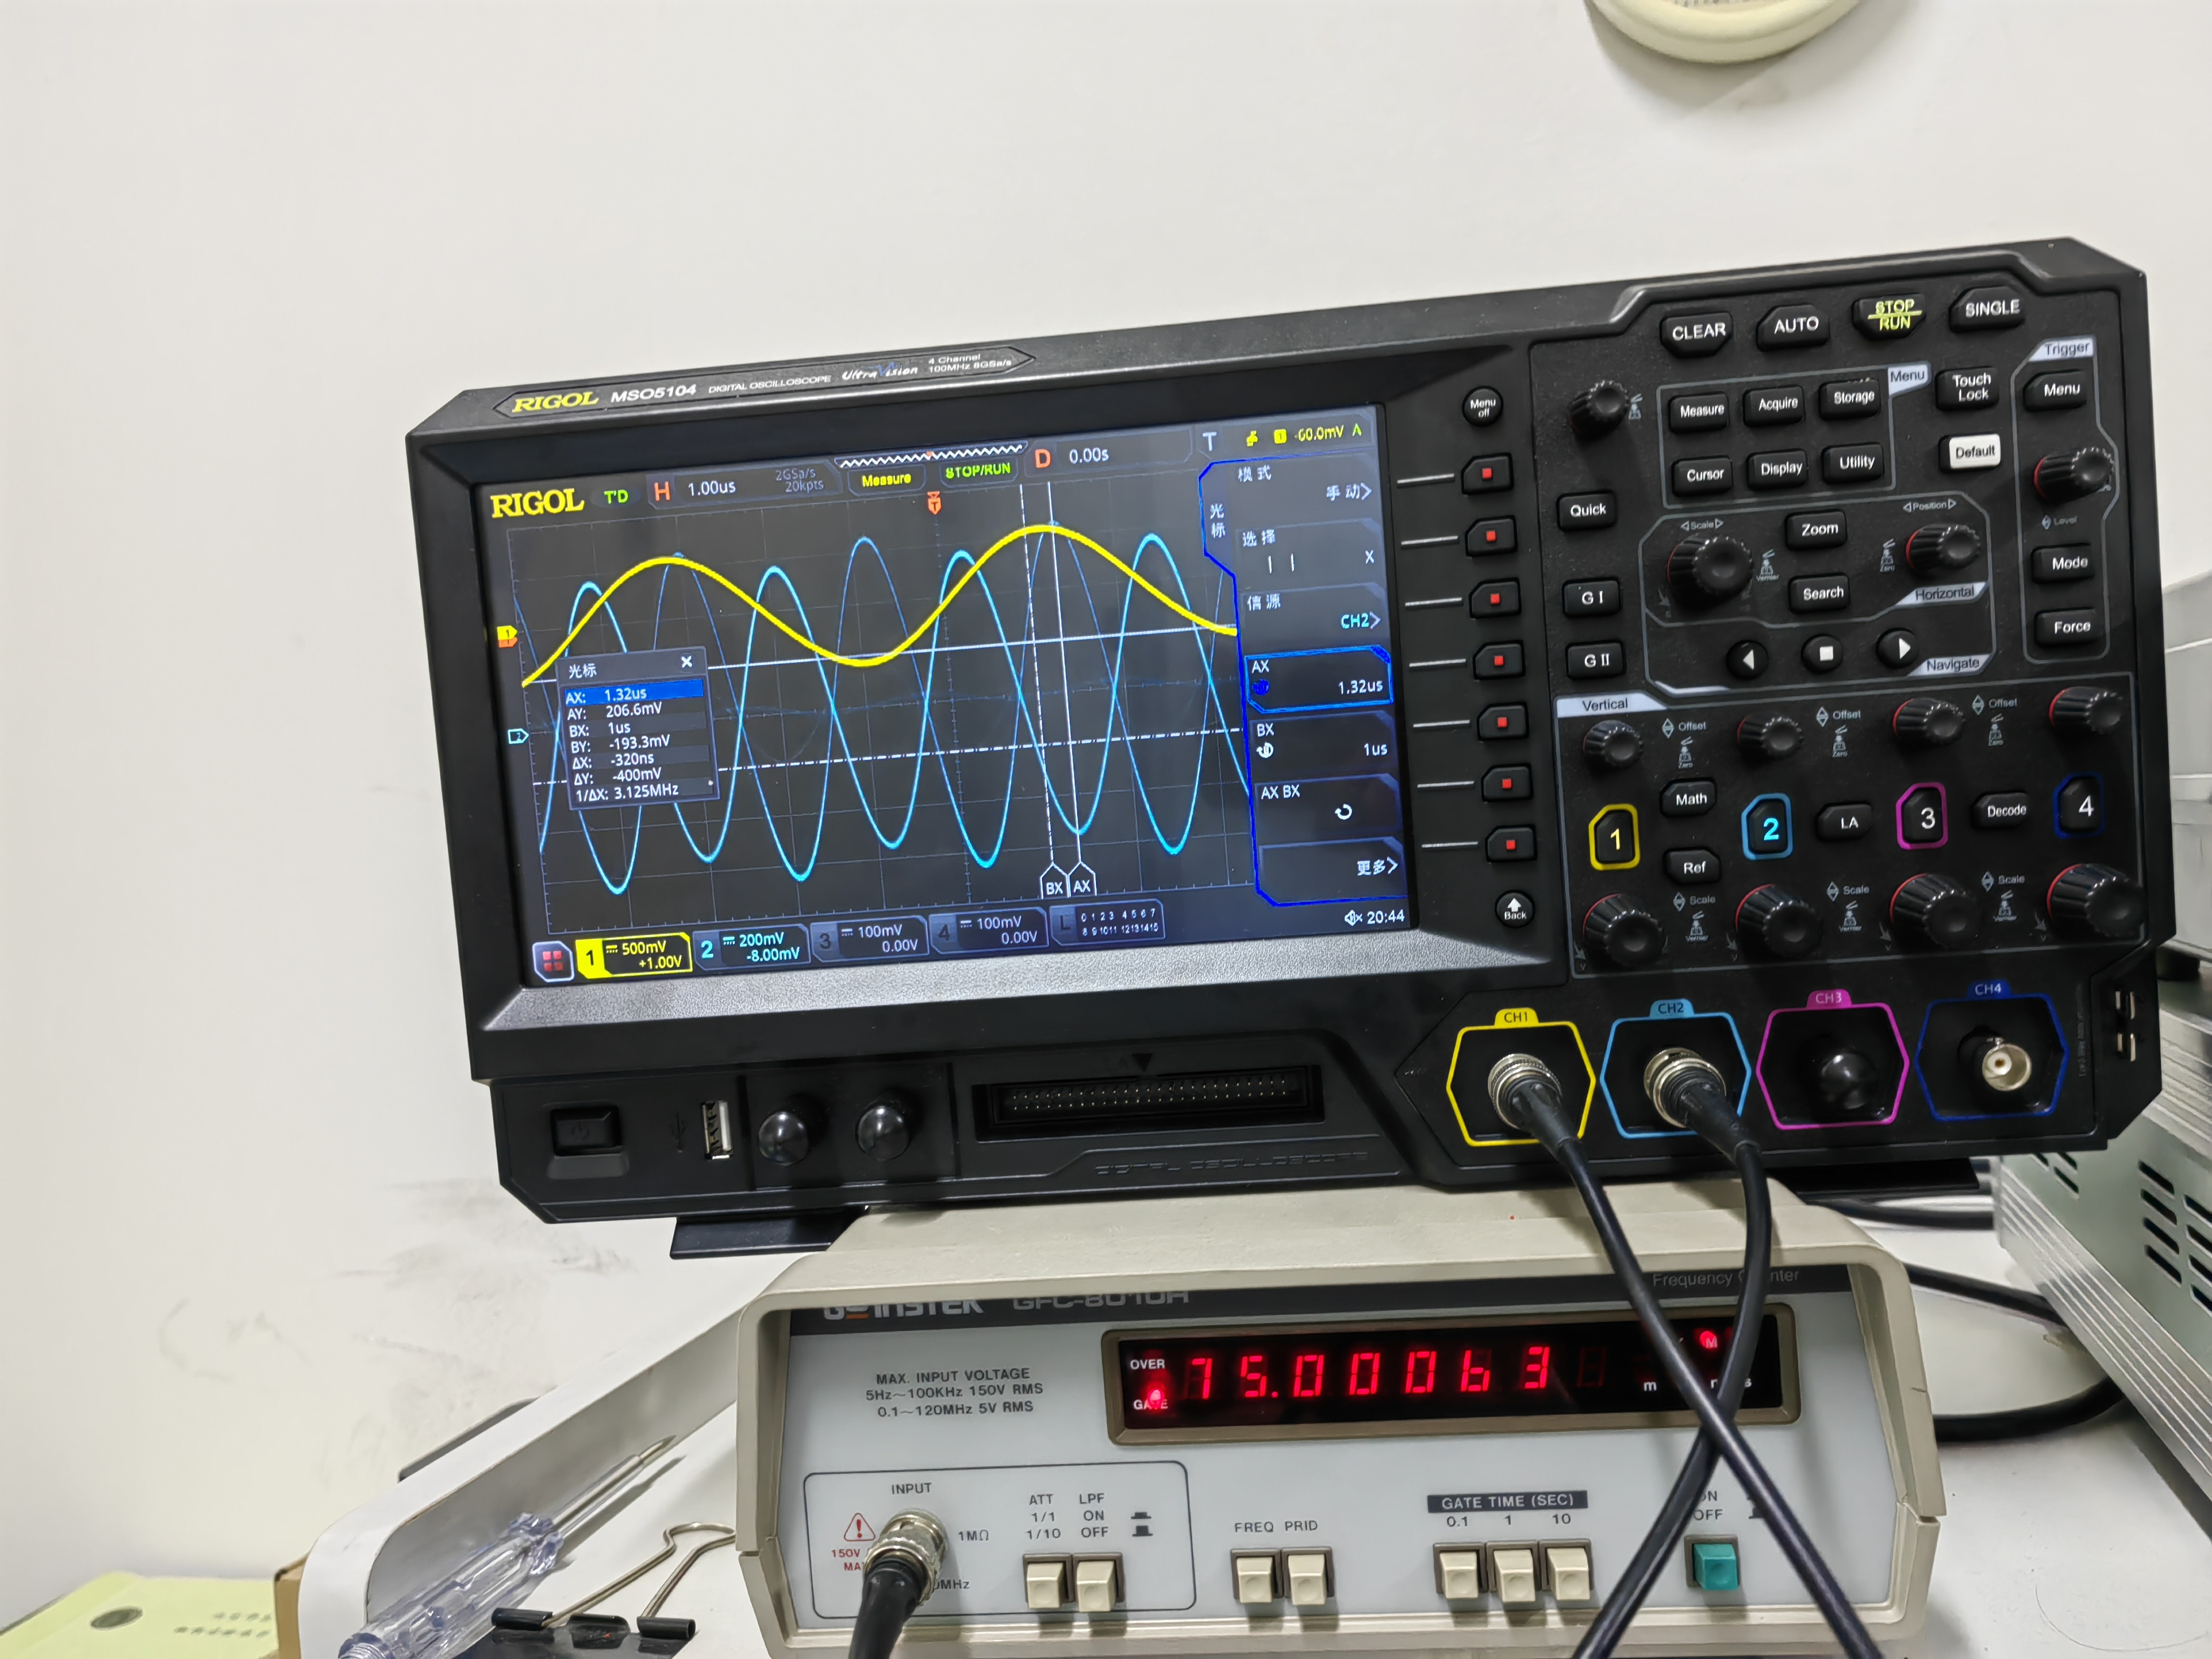
\includegraphics[width=0.7\textwidth]{2.jpg}
        \caption{相移$\pi$光强曲线示意图}
    \end{figure}
\section{总结}
本实验利用扫描干涉仪测量激光的纵模间距及由声光效应产生的0级,1级,2级衍射劈裂;
实验中测得激光的两纵模间距为619.03MHz,验证了超声波作用下纵模的劈裂满足$\Delta \nu=2\Omega$
使用光拍法测得光速的大小为$c=2.76\times 10^8m/s$。
\end{document}